\chapter{Distributed file systems}


\section{Definitions, architectural model and requirements}

A distributed file system enables persistent data storage throughout an intranet. The objective of a distributed file service is resource sharing in an effort to reduce costs of storage and data management. Examples of these file systems are \emph{Sun NFS} and the \emph{Andrew File System (AFS)}, which will be discussed later.

\emph{Files} form an elementary unit of a file system. A file consists of the actual data and a number of attributes, e.g. file length and timestamp. File naming is determined in \emph{directories} in which text names are mapped to file identifiers. Files can be managed and manipulated through a series of operations such as create, read and write.


\subsection{Design requirements}

When designing a distributed file system, a number of transparency requirements should be taken into account. For example: \emph{access transparency}, i.e., the set of operations for both local and remote files is the same, \emph{location transparency}, i.e., the representation of the file system does not reveal the physical location of the files, or \emph{mobility transparency}, i.e., when files are moved, no client code or administration tables should be altered.

Other requirements are for example maintaining file consistency, security (e.g. through Access Control Lists), concurrent file updates, replication and fault tolerance.


\subsection{Architectural model design}

The following architectural model is based on the implementation of both NFS and AFS. It considers three separate modules dividing responsibilities between them [1]:

\begin{itemize}
	\item \textbf{Flat file service} : Provides an implementation for operations on the file contents. \emph{Unique file identifiers (UFID)} are used to refer to files in all flat file service operations.
	\item \textbf{Directory service} : Provides a mapping between text names for files and their UFIDs and operations on directories.
	\item \textbf{Client module} : Provides a single programming interface for the flat file service and directory service and runs on a each client machine.
\end{itemize}

\textbf{Figure 1} gives a schematic overview of this model.


\begin{figure}
	\begin{center}
		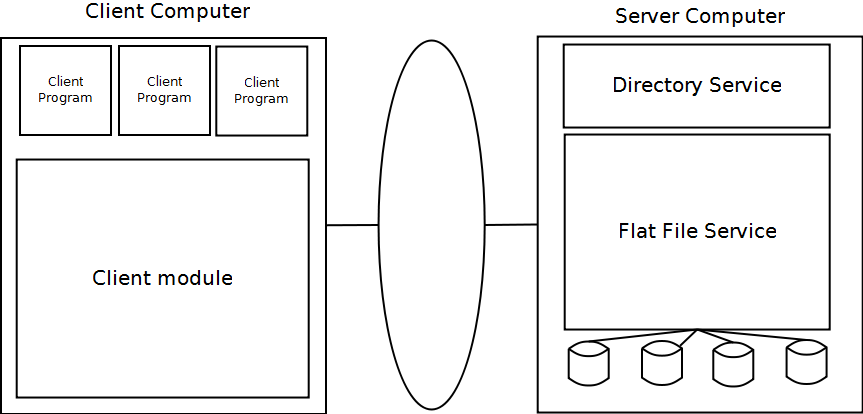
\includegraphics[width=0.7\textwidth]{img/fileservicearchitecture}
	\end{center}
	\caption{File service architecture.}
	\label{fig:fileservicearchitecture}
\end{figure}


\begin{table}
	\caption{Flat file system API, adapted from [1].}
	\label{tab:api:flatfilesystem}
	\begin{tabular}{p{150px} | p{250px}}
		\textbf{Operation} & \textbf{Description} \\
		\hline
		Read(FileId, i, n) $\rightarrow$ Data - throws BadPosition 	& \emph{If $1 \leq i \leq Length(File)$ : Reads a sequence of up to n items from a file starting at item i and returns it in Data.} \\
		Write(FileId, i, Data) - throws BadPosition 						& \emph{If $1 \leq i \leq Length(File)+1$ : Writes a sequence of Data to a file, starting at item i, extending the file if necessary.} \\
		Create() $\rightarrow$ FileId 																& \emph{Creates a new file of length 0 and delivers a UFID for it.} \\
		Delete(FileId) 																					& \emph{Removes the file from the file store.} \\
		GetAttributes(FileId) $\rightarrow$ Attr 										& \emph{Returns the file attributes for the file.} \\
		SetAttributes(FileId, Attr & \emph{Sets the file attributes.} \\
		\hline
	\end{tabular}
\end{table}


\begin{table}
	\caption{Directory service API, adapted from [1].}
	\label{tab:api:directoryservice}
	\begin{tabular}{p{150px} | p{250px}}
		\textbf{Operation} & \textbf{Description} \\
		\hline
		Lookup(Dir, Name) $\rightarrow$ FileId - throws NotFound 	& Locates the text name in the directory and returns the relevant UFID. If Name is not in the directory, throws an exception. \\
		AddName(Dir, Name, FileId) - throws NameDuplicate 				& If Name is not in the directory, adds (Name, File) to the directory and updates the file's attribute record. If Name is already in the directory, throws an exception. \\
		UnName(Dir, Name) - throws NotFound 											& If Name is in the directory, removes the entry containing Name from the directory. If Name is not in the directory, throws an exception. \\
		GetNames(Dir, Pattern) $\rightarrow$ NameSeq 							& Returns all the text names in the directory that match the regular expression Pattern. \\
		 &  \\
		 &  \\
		\hline
	\end{tabular}
\end{table}


\subsection{Implementation techniques}

\subsubsection{File groups}

A file group is a collection of files mounted on a given server. A server can contain multiple file groups. File groups can be transferred between servers and forms a unit of distribution over servers allowing transparent migration of file groups.

Files are locked in a file group on creation and are assigned a UFID including a file group identifier component [1,2]. File group identifiers are unique throughout the distributed system.

Examples of file groups are \emph{filesystems} (as opposed to \emph{file systems}) on NFS and \emph{volumes} on AFS.


\subsubsection{Space leak prevention}

The creation of a file is a two-step process [2]:
\begin{enumerate}
	\item Creation of an (empty) file with a new UFID;
	\item Naming of the file and adding the UFID to the corresponding directory;
\end{enumerate}

A failure after the first step causes the file to exist in the file server, but makes it unreachable, as the UFID is not in any directory. This lost space on disk is called a space leak. Detection of space leaks requires co-operation between the file server and the directory server [2].


\subsubsection{Access control}

Access control is required for security reasons. Access control models usually follow the model outlined by Lampson. Different abstraction models can be used to implement access control, e.g. proection domains, capabilities, access control lists, and so on [1].

Capabilities are binary values that act as digital keys. Ownership of a capability grants access to certain resources [1]. Capabilities are prone to two issues [1]:
\begin{enumerate}
	\item \textbf{Key theft} : Stolen keys can be abused regardless who its current owner is;
	\item \textbf{Revocation} : Users that are no longer authorized may still keep the key and use it maliciously;
\end{enumerate}


\subsubsection{Replication}

A file may be represented by a list of copies at different locations. This way servers can share the load, improving scalability and fault tolerance [1].


\subsubsection{Caching}

Server caching is used to reduce delay for disk I/O. Client caching reduces network delay [2].



\section{Example systems}

\subsection{Sun NFS}

\textbf{Figure 2} gives a schematic overview of the Sun NFS architecture. Note the similarity with the model depicted in \textbf{figure 1}.

In Sun NFS client and server modules can be in any node. Sun NFS attempts to emulate a standard file system by integrating file and directory services and integrating remote file systems in a local one through mounting [2]. This way Sun NFS tries to achieve access transparency.


\begin{figure}
	\begin{center}
		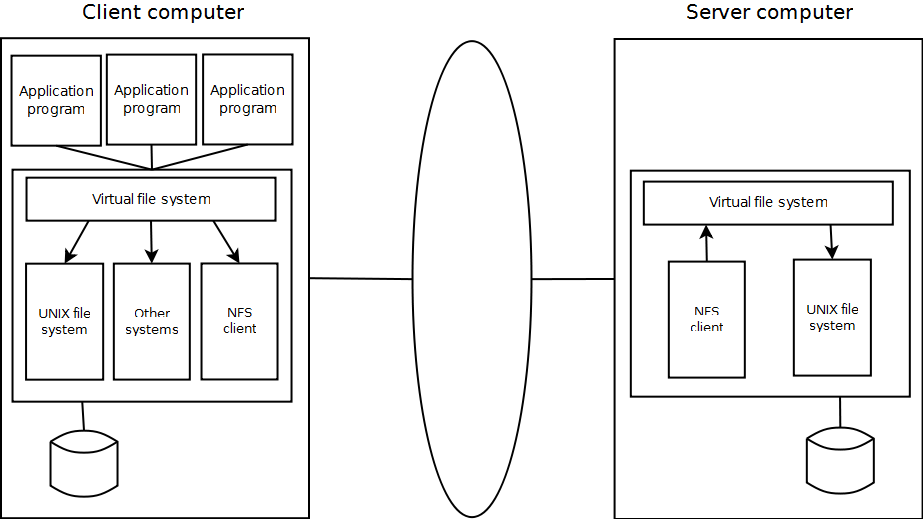
\includegraphics[width=0.7\textwidth]{img/nfs}
	\end{center}
	\caption{Sun NFS architecture.}
	\label{fig:nfs}
\end{figure}



\subsubsection{Virtual file system}

Sun NFS tries to achieve access transparency through a \emph{virtual file system (VFS)} that provides an abstraction layer on top of local and remote files. \textbf{Figure 2} illustrates the VFS layer providing access transparency for client applications [1].

The VFS is part of the UNIX kernel to manage local file identifiers and remote file identifiers, called \emph{file handles}. A file handle is a combination of the filesystem identifier, the i-node number and the i-node generation number. The i-node number of a UNIX file is an identification within the system that the file is stored. The i-node generation number reflects the number of times the i-node number has been reused [1].


\subsubsection{Integration through interfaces}

The NFS client module is integrated in kernel and offers a standard UNIX interface. This has several advantages [2]:
\begin{itemize}
	\item No client recompilation/reloading;
	\item Single client module for all user level processes;
	\item Encryption at kernel level.
\end{itemize}

Server integration is mainly implemented for performance reasons.

In the model depicted in \textbf{figure 2} is connected to the VFS in both client and server. Communication between client and server occurs through the interface and NFS protocol.


\subsubsection{Mounting service}

The mount service is a process that runs on the NFS server. The file \emph{/etc/exports} contains the names of the local filesystems that are avilable for remote mounting. Access lists determine which hosts are permitted to mount which filesystems. Users can mount any subtree of the filesystems they have access to, based on a chosen directory [1].

Remote filesystems may either be hard-mounted or soft-mounted in a client computer [1,2]:
\begin{itemize}
	\item \textbf{Hard-mounting} : A client waits until a request for a remote file succeeds;
	\item \textbf{Soft-mounting} : Mounting failure is returned if the request does not succeed after \textit{n} retries;
\end{itemize}

At the client, multi-part file pathnames are translated to i-node references. Each i-node referencing a remote mounted directory is translated into a file handle using a separate \textit{lookup()} request to the remote server. The VFS resolves file handles to local or remote directories. Mounting performance is improved through caching [1].

An addition to this system is the automounter. The automounter dynamically mounts remote directories when an empty mount point is referenced by a client. The automounter behaves as a local NFS server for the client machine. It holds a mapping of pathnames, or \emph{mount points} against corresponding servers. As the client accesses mount points when resolving a path name, the client module invokes a \textit{lookup()} request on the local automounter. The automounter triggers a number of probe requests to the corresponding NFS servers. Finally the referenced file systems are mounted onto the mount points via a symbolic link to avoid redundant requests to automounter [2].


\subsubsection{Caching}

Caching is done both at client and server side. Caching improves the performance of NFS significantly.

\paragraph{Server caching}

The server caching system is based on standard UNIX caching. File pages, directories, and file attributes read from disk are maintained in a memory buffer cache until the buffer space is required for other pages. Requests for files that are already in the cache then don't require expensive disk access. \emph{Read ahead} anticipates future read requests by fetching nearby file pages from memory [1].

When writes are performed in this system, additional measures are needed. The system supports two modes of writing [1]:
\begin{itemize}
	\item \textbf{Write-through} : The server writes updated file pages in the server's cache to disk before sending a reply to the client. When the reply is received, the client knows the data has been written to disk;
	\item \textbf{Delayed write} : Data stored in the cache is only written to memory when a commit operation is received for the relevant file. The client knows the file is written to disk as soon as a reply is received to a commit operation request;
\end{itemize}



\paragraph{Client caching}

Caching is used to reduce the number of requests to the server. The results of the following operations are cached: \textit{read()}, \textit{write()}, \textit{getattr()}, \textit{lookup()}, and \textit{readdir()}. As a result of the delayed updates introduced by caching, different versions of the same file pages may exist simultanously at different client nodes. To solve this problem, clients use polling to check the currency of their cached data, using a timestamp based method [1].

Let \textit{Tc} be the time when the cache entry was last validated, and \textit{Tm} the time when the block was last modified at the server. A cache entry is valid at time \textit{T} if \textit{T - Tc} is less than a freshness interval \textit{t}, or if the value for \textit{Tm} recorded at the client is equal to this value recorded at the server. The value of the freshness interval \textit{t} is a tradeoff between consistency and efficiency - on a Sun Solaris client, \textit{t} lies somewhere between 3 and 30 seconds. Formally this yields to following formula:

$(T - Tc < t) \vee (Tm_{client} = Tm_{server})$ \\

The cause for recent updates not to be visible immediately at the client has two sources of delay:
\begin{itemize}
	\item The delay after the write before the updated data leaves the cache in the updating client's kernel;
	\item The window for cache validation.
\end{itemize}

When a cached page is modified, it is marked as dirty and scheduled to be flushed to the server asynchronously. Pages are flushed when a file is closed or a \textit{sync} operation occurs at the client. A \emph{bio-daemon} is used to facilitate read-ahead and delayed-write operations. A bio-daemon is notified after each read request, and it requests the transfer of the following file block from the server to the client cache. In the case of writing, the bio-daemon will send a block to the server whenever a block has been filled by a client operation [1].


\subsubsection{Access control}

The NFS server is stateless. As a result, the user's identity has to be verified against the file's access permission attributes with each request. Encryption and integration with Kerberos tries to prevent impersonation [1].







\subsection{Andrew File System}

A schematic overview of the Andrew File System is given in \textbf{figure 3}.

\begin{figure}
	\begin{center}
		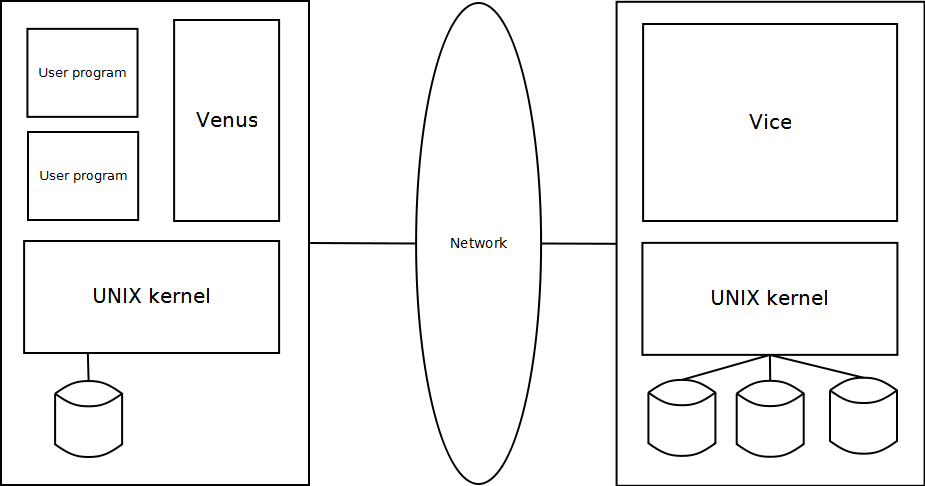
\includegraphics[width=0.7\textwidth]{img/afs}
	\end{center}
	\caption{Andrew File System architecture.}
	\label{fig:afs}
\end{figure}


The Andrew File System is characterized by two design decisions [1]:
\begin{enumerate}
	\item \textbf{Whole-file serving} : The entire file contents are transmitted to client computers by AFS servers;
	\item \textbf{Whole-file caching} : File copies at the client are stored in a cache on the local disk, i.e., the cache is permanent.
\end{enumerate}

The design strategy is based on a number of assumptions about the average and maximum file size and locality of reference to files in UNIX systems [1]:
\begin{itemize}
	\item Files are small;
	\item Read operations are much more common than write operations;
	\item Sequential access is common, random writes are rare;
	\item Most files are read and written only by one user;
	\item Files are referenced in bursts, i.e., files referenced recently are likely to be referenced again.
\end{itemize}

A scenario that illustrates the operation of AFS is as follows [1]:
\begin{enumerate}
	\item The user process in a client computer issues an \textit{open} call for a file the shared file space. There is no current copy of the file in the cache. The client sends a request to the server containing the file.
	\item The copy is stored in the local UNIX file system in the client computer. The copy is opnened and the resulting UNIX file descriptor is returned to the client.
	\item Subsequent \textit{read}, \textit{write}, etc. operations on the file by processes in the client computer are applied on the local copy.
	\item The client process issues a \textit{close} system call. If the local copy has been updated, its contents are sent back to the server. The server performs relevant updates. The client keeps its copy of the file in the cache.
\end{enumerate}

The design affects performance and the semantics of the system. Based on the previously described design characteristics, we can make the following predictions about AFS performance:
\begin{itemize}
	\item Locally cached copies remain valid for a long time if the files are updated infrequently and/or files that are updated by just a single user;
	\item The provision of sufficient cache space on a client machine ensures that files in regular use are normally retained in the cache until they are needed again;
	\item Databases do not scale well with AFS as they are updated frequently and shared by many users.
\end{itemize}



\subsubsection{Implementation}

The \emph{Vice} is server software that runs as a user-level UNIX process in each server computer. The \emph{Venus} is a user-level process that runs in the client computer. Referring to the abstract model in \textbf{figure 1}, the Venus process corresponds to the client module [1].

File in the workstations are either local or shared. Shared files are stored on servers and copies are cached in client computers. A specific subtree \textit{cmu} contains all the shared files. User directories are in the shared space, enabling file access from any workstation. One of the partitions on the local disk of each workstation is used as a cache. It is managed by the Venus component of the client [1].

Files are grouped into volumes. \emph{Fids} include the volume number of the volume containing the file, an NFS file handle identifying the file within the volume, and a \textit{uniquifier} to avoid fid reuse. The Vice servers only accept requests by the Venus in terms of fids. On the client computer pathnames are used to access files, which are then translated by the Venus component into fids [1].



\subsubsection{Caching}

When Vice supplies a copy of a file to a Venus process it also provides a callback promise. A \emph{callback promise} is a token issued by the Vice server that is the custodian of the file, guaranteeing that it will notify the Venus process when any other client modifies the file [1].

Whenever the client's Venus handles an \textit{open} operation, it checks the cache. If the required file is found in the cache, then its token is checked. The token can have two states [1]:
\begin{itemize}
	\item \textbf{Valid} : The cached copy can be opened and used without reference to Vice;
	\item \textbf{Cancelled} : A fresh copy of the file must be fetched from the Vice server. When the Venus process receives a callback, it sets the callback promise token for the relevant file to cancelled.
\end{itemize}


\paragraph{Maintaining consistency}

When a workstation is restarted after a failure or a shutdown, its Venus component cannot assume that the callback promise tokens are correct, as some callbacks may have been missed. So before a file is accessed, the Venus has to send a validation request containing the file modification timestamp to the server that is the custodian of the file. If the timestamp is current, the server responds with valid and the token is reinstated. If the timestamp shows that the file is out of date, then the server responds with cancelled and the token is set to cancelled [1].

To deal with possible communication failures, e.g., loss of callback messages, callbacks must be renewed before an \textit{open} operation if a certain amount of time has passed since the file was cached without communication from the server.

Since the majority of files are not accessed concurrently, and read operations predominate over writes in most applications, the callback mechanism results in a dramatic reduction in the number of client-server interactions [1].

The callback mechanism used in AFS requires Vice servers to maintain some state on behalf of their Venus clients, unlike NFS. To retain callback lists must be retained over server failures, they are held on the server disks and are updated using atomic operations. This design decision introduces some overhead: dealing with failures, maintaining state.


\paragraph{Update semantics}

One-copy file semantics are not practicable in large-scale systems. A strict implementation of one-copy semantics would require that the results of each write to a file are distributed to all cached copies before any further accesses can occur. The goal of the cache-consistency mechanism is to achieve an approximation of these semantics [1].

A client may open an old copy of a file after it has been updated by another client. This occurs if a callback message is lost, for example as a result of a network failure. But there is a maximum time, \textit{T}, for which a client can remain unaware of a newer version of a file. For a client \textit{C}, a file \textit{F} and corresponding custodian server \textit{S} we have the following guarantee after a successful \textit{open}:

$latest(F, S, 0) \vee (lostCallback(S, T) \wedge inCache(F) \wedge latest(F, S, T))$ \\

Here \textit{latest}(\textit{F}, \textit{S}, \textit{T}) denotes that the copy of \textit{F} seen by the client is no more than T seconds out of date, \textit{lostCallback}(\textit{S}, \textit{T}) denotes that a callback message from \textit{S} to \textit{C} has been lost at some time during the last \textit{T} seconds, and \textit{inCache}(\textit{F}) indicates that the file \textit{F} was in the cache at \textit{C} before the open operation was attempted [1].


\section*{References}

\begin{enumerate}[1]
	\item G. Coulouris, J. Dollimore, T. Kindberg and G. Blair, "Distributed Systems: Concepts and Design (5th Edition)", M. Horton, Red., Addison-Wesley, 2011, p. 1063.
	\item W. Joosen, 2013, "Distributed File Systems", iMinds-DistriNet KULeuven
\end{enumerate}